\documentclass[preprintnumbers,amsmath,amssymb,superscriptaddress,twocolumn,showpacs]{revtex4-2}
\usepackage{graphicx}% Include figure files
\usepackage{dcolumn}% Align table columns on decimal point
\usepackage{bm}% bold math
\usepackage{natbib}
\usepackage{physics}
\usepackage[caption=false]{subfig}



%\newcommand{|}{Y$_2$SiO$_5$}
\def\sgn{\mathop{\rm sgn}}
\newcommand{\be}{\begin{equation}}
\newcommand{\ee}{\end{equation}}
\newcommand{\bea}{\begin{eqnarray}}
\newcommand{\eea}{\end{eqnarray}}

\begin{document}

\title{Low field depolarization of electronic spins through dipole-dipole coupling}

\author{C. Pellet-Mary$^1$, M. Perdriat$^1$, G. H\'etet} 

\affiliation{Laboratoire De Physique de l'\'Ecole Normale Sup\'erieure, \'Ecole Normale Sup\'erieure, PSL Research University, CNRS, Sorbonne Universit\'e, Universit\'e Paris Cit\'e , 24 rue Lhomond, 75231 Paris Cedex 05, France.}

\begin{abstract}
C'est trop bien
\end{abstract}

\maketitle
Blabla sur les NV, les ensembles etc.


%réécrire le début et foutre la partie sur la PL avant le T1. Peut-etre dans le blabla sur les ensembles justement

%We have identified three mechanisms for the low field depolarization, two of which have not been reported before.

\begin{figure}
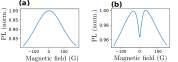
\includegraphics[width=0.45\textwidth]{Figures/fig dense vs pas dense}
\caption{Photoluminescence from NV centers as a function of an external magnetic field randomly oriented for two samples : (a) a CVD sample containing $\approx$ 4 ppb NV$^-$ centers, (b) an HPHT sample containing $\approx$ 3 ppm NV$^-$ centers}
\label{PL_NV_density}
\end{figure}

In this letter/article, we characterize the depolarization of the spins observed for dense ensemble of NV centers in zero magnetic field and its potential application for DC magnetometry. While the main mechanism behind the depolarization, the lift in the degeneracy between the four classes of NV centers, is already well studied and can be exploited in a microwave-less vector magnetometry protocol, we found two other depolarization mechanisms specific to the zero-field region which could play an important role in a low-field magnetometry protocol.

The main signature of the spin depolarization in low field is the characteristic dip in photoluminescence (PL) observed only for high density ($\gtrsim 1$ ppm) of NV centers, as shown on fig \ref{PL_NV_density}. The decrease in the spins' lifetime in zero field makes the optical polarization scheme of the NV centers less effective and therefore reduce the population of the bright $\ket{0}$ spin state. %The reason for the decrease in PL at higher magnetic field values is the mixing of the bright spin state $\ket{0}$ to the darker state $\ket{-1}$ induced by the transverse magnetic field. This effect does not modify (on first approximation) the spins' lifetime, and is common to both dense and sparse samples.

\begin{figure}
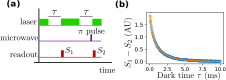
\includegraphics[width=0.45\textwidth]{Figures/fig T1}
\caption{Spin $T_1$ measurement protocol. (a) Sequence used to measure the spin lifetime : the laser is turned off for a time $\tau$ twice and the spin state is read at the end of the dark time by measuring the initial photoluminescence when the laser is turned back on. A microwave resonant with one of the spin transition is used in one of the sequence to project the $\ket{0}$ spin sate in either $\ket{+1}$ or $\ket{-1}$. The sequence result is the subtraction $S_1-S_2$. (b) Measurement of a dense ensemble spin lifetime in zero field and non-zero field, fitted with an expression $A \exp (-\frac{\tau}{T_1^{\rm ph}} -\sqrt{\frac{\tau}{T_1^{\rm dd}}})$}
\label{T1}
\end{figure}

The $T_1$ depolarization dynamics of single or sparse NV centers at room temperature is dominated by a two-phonon Raman process, which depends on the crystal lattice temperature but does not (?) depend on the external magnetic field. However, it has been observed that dense NV centers ensemble have an additional spin decay channel which depends greatly on the magnetic field and not on the temperature. This effect has been attributed to cross-relaxation between the NV centers through dipole-dipole coupling. Some inhomogeneity between the NV centers is further needed in order to explain the depolarization of the spin ensemble. We will denote $T_1^{\rm ph}$ the characteristic time associated with the phonon relaxation process and $T_1^{\rm dd}$ the characteristic time associated with the dipole-dipole relaxation process.

The spin lifetime protocol used here is described in Fig. \ref{T1} and is based on previous similar experiments. It consists in a pump-probe measurement where the spins are first polarized in the $\ket{0}$ state by a green laser, and read-out optically after a variable dark time $\tau$. Using only this sequence can result in artifacts in the signal, mostly due to charge state transfer in the dark \citep{giri_coupled_2018}. It is therefore convenient to repeat the sequence with an additional $\pi$ pulse right before the spin read-out to project the remaining $\ket{0}$ polarization into a darker $\ket{+1}$ or $\ket{-1}$ state. By subtracting the result of the two sequences, we select only the spin-dependent part of the signal, with the added benefit of being able to select a specific class of NV centers. 

The ensemble spin lifetime is non-exponential due to inhomogeneities between the NV$^-$ centers. We will base our interpretations of the experimental results on the NV-fluctuator model developed in \citep{choi_depolarization_2017}. A conclusion of this model is that, for an homogeneous 3D distribution of fluctuator, the dipole-induced lifetime should be stretched-exponential with a stretch factor $\beta=1/2$. Such an ensemble lifetime is indeed observed when $T_1^{\rm dd} \ll T_1^{\rm ph}$  (see SI).

For the samples used in this paper (detailed in SI), we observed that $T_1^{\rm dd} \sim T_1^{\rm ph}$, meaning that we had to include both  in our analysis. The resulting fitting formula is therefore :
\begin{equation}
S(\tau)=A \exp (-\frac{\tau}{T_1^{\rm ph}} -\sqrt{\frac{\tau}{T_1^{\rm dd}}}),
\end{equation}
In order to get comparable fitting parameters between each measurement, we decided to fix the value of the exponential lifetime in the fitting process, leaving only the stretch lifetime as a free parameter. For Fig.\ref{T1}, \ref{largeur_fluct}, \ref{100_VS_1x4} and \ref{exp_B_transverse}, the chosen exponential lifetime was $T_1^{\rm ph}=3.62 \ \rm ms$.

\begin{figure}
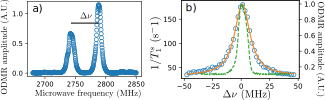
\includegraphics[width=0.45\textwidth]{Figures/fig largeur fluct}
\caption{Tuning resonant coupling through magnetic field orientation. (a) Sketch of the four possible orientations ("classes") in a single crystal diamond lattice. (b) ODMR spectrum showing four $\ket{0} \to \ket{-1}$ resonances corresponding to the four spin classes. The detuning $\Delta \nu$ between the classes $\beta$ and $\gamma$ was controlled by changing the orientation of the external magnetic field.(c) Stretch part of the lifetime decay for the spins resonant with $\nu_\gamma$ as a function of the detuning $\Delta \nu$ (blue circles), fitted by a Lorentzian with half width at half maximum 8.04 MHz . Green dashed line correspond to the ODMR width of a single class stretched by a factor $\sqrt 2$, approximating the overlap of the two classes (see SI).}
\label{largeur_fluct}
\end{figure}

Fig. \ref{largeur_fluct} illustrates how we can use the NV center geometry to tune the resonant dipolar-coupling between the spins. Because of the diamond symmetry, we can distinguish 4 groups ("classes") of identical NV centers, based on the four possible orientation of the NV axis in the crystal. These four classes have \textit{a priori} different spin resonance frequency based on the projection of the magnetic field on their respective NV axis. By tuning the angle of the magnetic field, we can therefore control the frequency detuning between the different classes, and as a result we can control the number of resonant NV centers by bringing in and out of resonance several classes.

Fig. \ref{largeur_fluct} (c) in particular shows the dipole-induced lifetime $T_1^{\rm dd}$ for a given class as a function of the energy detuning with another class. One can notice that the width of the $T_1^{\rm dd}$ bell shape is significantly larger than that of the frequency overlap between the two classes, modeled here by an ODMR line stretched by a factor $\sqrt{2}$ (see SI). This extra width can not be attributed to the dipole-dipole coupling strength : for a 3 ppm concentration of NV$^-$ centers, the average coupling strength between neighboring NV centers should be $\sim 27\ \rm kHz$, two order of magnitude below the observed width. We can also see that $T_1^{\rm dd}$ follows a Lorentzian shape despite the ODMR lines being non-Lorentzian. These two observations corroborate the idea developed in \cite{choi_depolarization_2017} that the interaction width is dominated by the noise spectrum of the lifetime-limited fluctuators.

\begin{figure*}
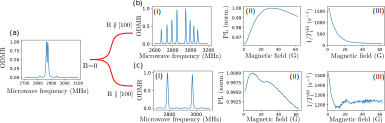
\includegraphics[width=.95\textwidth]{Figures/fig 100 vs 1x1x1x1}
\caption{Dependency of the magnetic field angle for the zero field depolarization. (a) ODMR spectrum in zero field. (b) ODMR spectrum for a magnetic field $\approx$ 60 G. The field is aligned (b2) or misaligned (b1, $\approx 24^\circ$ of misalignment) with the crystalline [100] direction. (c) Normalized photoluminescence of the NV$^-$ ensemble as a function of the magnetic field amplitude for the same field orientations as fig (b). (d) Stretch part of the lifetime decay as a function of the magnetic field amplitude for the same field orientations as fig (b).}
\label{100_VS_1x4}
\end{figure*}

The depolarization in low field can be explained in large part due to the lift of degeneracy between the four classes, as can be seen in Fig. \ref{100_VS_1x4} : On the top part, a magnetic field is scanned in a direction chosen in order to quickly split the transition frequencies of the four NV classes. We can observe an increase of about 4\% in the photoluminescence and an increase by a factor of $\sim$ 16 in the spin dipolar-induced lifetime ${T_1^{\rm dd}}$ as the magnetic field is increased.

However the splitting of the four classes can not explain entirely the spin depolarization in zero field. The bottom part of Fig. \ref{100_VS_1x4} shows a similar experiment when the magnetic field is aligned with the [100] crystalline axis. In this particular orientation, the projection of the magnetic field on the four NV classes is identical, meaning that the resonance condition between the NV centers remains the same in zero and non-zero field. Yet we can still observe an increase of $\sim$ 0.5\% in the photoluminescence and an increase of $\sim$ 30\% in ${T_1^{\rm dd}}$.
We attribute the remaining depolarization to two phenomena : the change of basis in the spin Hamiltonian's eigenstate in zero-field, and the near-resonance of the dipolar double-flip processes.

The decrease of spin lifetime and the associated drop in PL for $B\approx 20\ \rm G$ is due to cross-relaxations between NV $^-$ centers with a $^{13}$C as first a neighbor, and those without \cite{pellet2021optical}.

The dipole-dipole interaction Hamiltonian between two spins ${\vec S}_1$ and ${\vec S}_2$reads :
\begin{equation}
\mathcal{H}^{\rm dd}= -\frac{J_0}{r^3}\left(3\left({\vec S}_1 \cdot \vec u \right)\left({\vec S}_2 \cdot \vec u \right) - {\vec S}_1 \cdot {\vec S}_2  \right),
\end{equation}
Where $J_0= (2 \pi) 52\ \rm MHz \cdot \rm{nm}^3$, $\vec r$ is the relative positions of the two spins and $\vec u = \frac{\vec r}{\norm{\vec r}}$. In situations such as the one described in Fig. \ref{largeur_fluct}, the only relevant terms of $\mathcal{H}^{\rm dd}$ in term of population transfer are the flip-flop terms such as $\mel{0,+1}{\mathcal{H}^{\rm dd}}{+1,0}$. In zero magnetic field however, we have to take into account other aspects of the dipolar Hamiltonian in consideration.

First is the change of basis of the single spin Hamiltonian $\mathcal{H}_s$ : in zero external magnetic field, the eigenstates of $\mathcal{H}_s$ in the $\{\ket{+1},\ket{-1}\}$ manifold are determined by local electric and magnetic field coming from nearby impurities \cite{mittiga2018imaging}. For the samples used in this study, $\mathcal{H}_s$ was dominated by local electric field (see SI), meaning that the proper eigenstates of $\mathcal{H}_s$ in zero magnetic field are $\{ \ket{0},\ket{+}=\frac{\ket{+1}+\ket{-1}}{\sqrt{2}},\ket{-}=\frac{\ket{+1}-\ket{-1}}{\sqrt{2}} \} $

Because the splitting between $\ket{+}$ and $\ket{-}$ ($\approx 9\ \rm MHz$) is much greater than the dipole-dipole interaction ($J_0 / r^3 \approx 30\ \rm kHz$), the flip-flop terms of $\mathcal{H}^{\rm dd}$ now reads $\mel{0,+}{\mathcal{H}^{\rm dd}}{+,0}$. Averaging over all relative positions of two aligned NV centers, we found that on average $\abs{\mel{0,+}{\mathcal{H}^{\rm dd}}{+,0}}$ was greater than 
$\abs{\mel{0,+1}{\mathcal{H}^{\rm dd}}{+1,0}}$ by a factor $1.8 \sim 2$ depending on the correlation lengths of the local electric field.
When all four classes are resonant, the theoretical decrease in the spin lifetime due to the change of basis is $\sim 20 \%$ (See SI de ouf).

Second is the near-resonance condition of the double-flip processes such as $\mel{0,+1}{\mathcal{H}^{\rm dd}}{-1,0}$ or $\mel{0,+}{\mathcal{H}^{\rm dd}}{-,0}$. These terms usually couple non resonant states due to the energy mismatch between $\ket{+1}$ and $\ket{-1}$. However in zero field, the energy splitting between $\ket{+}$ and $\ket{-}$ is comparable with the fluctuator's spectral width measured in Fig. \ref{largeur_fluct} to be $\approx 8\ \rm MHz$, making the double-flip population transfer possible.

\begin{figure}
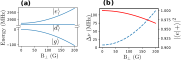
\includegraphics[width=0.45\textwidth]{Figures/fig transverse field simu}
\caption{Simulated eigenstates of the spin Hamiltonian in the presence of purely transverse magnetic field. (a) Energies of the three eigenstates $\ket{g}$, $\ket{d}$ and $\ket{e}$ as a function of the magnetic field amplitude. (b) Blue dashed curve : frequency detuning between the two transitions $\ket{g} \leftrightarrow \ket{d}$ and $\ket{g} \leftrightarrow \ket{e}$. Plain red curve : projection of $\ket{e}$ on $\ket{+}=(\ket{+1}+\ket{-1})/\sqrt{2}$ as a function the magnetic field. Is equal to the projection of $\ket{g}$ on $\ket{0}$.}
\label{calculs_B_transverse}
\end{figure}

In order to evaluate the relative contribution of these two factors, we investigate the spin relaxation in the case of pure transverse magnetic field. Calling $\{ \ket{g}, \ket{d}, \ket{e} \}$ the three eigenstates of the spin Hamiltonian in the presence of purely transverse magnetic field, Fig. \ref{calculs_B_transverse} shows that for small enough magnetic field, the $\{ \ket{g}, \ket{d}, \ket{e} \}$ basis is almost equal to the $\{ \ket{0},\ket{+},\ket{-} \} $ basis : for $B=120\ \rm G$, $\braket{0}{g}\approx 0.99$, $\braket{-1}{d}=1$ and $\braket{+1}{e}\approx 0.99$. However the energy difference between $\ket{d}$ and $\ket{e}$ reaches $\approx 45\ \rm G$ which is high enough to cancel out the double-flip processes and allows us to isolate the change of basis hypothesis from the double-flip one.
%As shown in Fig. SOON, (and in SI), the $\{ \ket{0},\ket{+},\ket{-} \} $ basis correspond to the spin Hamiltonian eigenstates in two situations : either in zero magnetic field when the electric field dominates, or when the magnetic field is purely transverse, as long as it remains small before the zero-field splitting. %(rq : est-ce que je dois mettre le hamiltonien de spin dans le main text du coup ?).

\begin{figure}
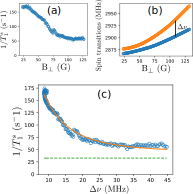
\includegraphics[width=0.45\textwidth]{Figures/fig transverse field}
\caption{Modification of the stretch lifetime in the presence of purely transverse magnetic field. (a) Stretch component of the ensemble lifetime as a function of the field amplitude. (b) Transition frequencies for the $\ket{g} \leftrightarrow \ket{d}$ and $\ket{g} \leftrightarrow \ket{e}$ transitions, measured through ODMR. (c) Stretch component of the lifetime as a function of the frequency detuning between the two transistions (blue circles), fitted by a Lorentzian centered in $\Delta \nu=0$ with half width at half maximum 8MHz. The green dashed line correspond to the lifetime of a single class aligned with the magnetic field.}
\label{exp_B_transverse}
\end{figure}

Fig. \ref{exp_B_transverse} shows the dipole-dipole spin relaxation $T_1^{\rm dd}$ for a class of NV whose axis is orthogonal to the applied magnetic field. By monitoring the frequencies of the transitions $\ket{g} \leftrightarrow \ket{d}$ and $\ket{g} \leftrightarrow \ket{e}$, we can deduce the detuning $\Delta \nu$ between the two-spin states $\ket{0,+}$ and $\ket{-,0}$. Plotting then $1/T_1^{\rm dd}$ as a function of $\Delta \nu$, we can notice two things. 

First the decrease of $1/T_1^{\rm dd}$ as $\Delta \nu$ increases which corresponds to the loss in effectiveness of the double flip processes. The shape of the curve matches decently well with the tail of a Lorentzian centered in $\Delta \nu=0$ with a width of 8 MHz, confirming that the double-flip process interaction range is likely determined by the fluctuators noise spectrum just like the flip-flop processes. 

Second is the plateau reached for $\Delta \nu \gtrsim 30\ \rm MHz$. The final $1/T_1^{\rm dd}$ value is about twice as high as that for a spin well aligned with the magnetic field, showing the increased depolarization due to the change of basis.

This experiment shows that, for the sample studied here, the depolarization due to the double-flip processes dominates the one due to the change of basis in zero magnetic field.

\section*{Magnetometry}
\begin{figure}
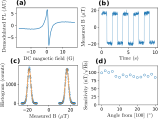
\includegraphics[width=0.45\textwidth]{Figures/fig_magneto}
\caption{Low field magnetometry protocol. (a) Demodulated photoluminescence as a function of an externally applied magnetic field with an additional oscillatory magnetic field. (b) Measured magnetic field when alternating a small external magnetic field offset. (c) Histogram of the measurement in Fig. (b) fitted with gaussians of standard deviation $\sigma=1.5\ \mu \rm T$}. (d) Measured sensitivity as function of the angle between the external magnetic field and the [100] crystalline axis.
\label{magneto}
\end{figure}
DC microwave-less magnetometry has already been performed with NV ensembles, using either cross-relaxations [les russes] or level anti-crossing [bubu]. Here we propose to perform a similar protocol, but using the spin depolarization in zero-field. The main difference with the previously mentioned protocols is the fact that this one doesn't rely on crystalline orientation, making this protocol usable with diamond powders or polycrystalline samples.

Fig. \ref{magneto} (a) shows the demodulated PL when a DC magnetic field is scanned in a random direction and an additional alternating magnetic field of a few Gauss at $\sim \ \rm kHz$ is added through the same electromagnet (see experimental details in SI). We can see a sharp and relatively linear slope in low field $\abs{B} < 5\ \rm G$. Once calibrated, in this case with ODMR, the slope can provide a 1D magnetic field measurement, which could be extended to 3D with a set of 3 coils or 3 electromagnets, as seen in \cite{zheng_microwave-free_2020}.

In order to measure the sensitivity of the measurement, we alternate a small DC field of $\approx 40 \rm G$ every few seconds and take an histogram of the measured fields, as shown in Fig. \ref{magneto} (b) and (c). The histogram is well fitted with gaussians of standard deviation $\sigma=1.5\ \mu \rm T$. The measurement was performed here with an output low-pass filter of time constant $\tau=3\ \rm ms$, which allows us to measure the sensitivity $\eta=\sigma \sqrt{\tau}=82\ \rm{nT}/\sqrt{\rm Hz}$.

We can then try to measure the relative importance of the three causes of spin depolarization on the field sensitivity. In order to do so, we measure the sensitivity while changing the angle of the field. When $\vec B$ is aligned with the [100] crystalline axis, only the double flips and the change of basis are present, whereas in every other orientation the three effects are at play.

The results are shown in Fig. \ref{magneto} (d). We can see a slight increase of $\sim$ 10\% in the sensitivity as we leave the [100] region, but overall the sensitivity remains relatively flat, which means that the double-flips and change of basis effects are the dominant factors in the sensitivity of this protocol. %This is in agreement with the measurements in Fig. \ref{100_VS_1x4} : even though the contrast is much better in the not-[100] case, the slope in term of contrast percentage/magnetic field is comparable in both cases (en faite pas complètement, y'a pas loin d'un facteur 2 sur les dérivées numériques)
It should be noted though that this observation is sample dependent, and that other samples, including from the same batch, have shown a higher orientation dependence, corresponding to a lower contribution from the double flips and change of basis.

\section*{Conclusion}
In this work we have identified three mechanisms causing the extra spin depolarization observed in zero field for dense ensemble of NV$^-$ centers, all related to an increase in the dipole-dipole cross-relaxations between the spins : the lift of degeneracy between the four classes caused by the magnetic field, the change of basis in the spin Hamiltonian when the transverse electric field becomes dominant, and the double-flip process allowed by the proximity in energy of the spin $\ket{\pm}$ states. We identified the lift in degeneracy as the main cause in the zero-field depolarization, followed by the double-flip process and then the change of basis. With have demonstrated a potential use of this depolarization as a DC microwave-less and orientation-free magnetometer with senstivity below $100\ \rm{nm}/\sqrt{\rm Hz}$ for a single $10\ \mu \rm m$ crystal.We have observed that in some cases the double-flips and change of basis depolarization play a more important role than the lift of degeneracy in the low field sensitivity.
\section*{acknowledgements}

\bibliographystyle{plain}
\bibliography{CR}{}



\end{document}